\documentclass[tikz,border=20pt]{standalone}
\usetikzlibrary{shapes,calc,arrows.meta}
\usepackage{xcolor}

\definecolor{bgcream}{HTML}{FCF6EE}
\definecolor{bearbrown}{HTML}{C98F55}
\definecolor{beardark}{HTML}{A87139}
\definecolor{bearcream}{HTML}{FAEBD7}
\definecolor{stitchcolor}{HTML}{9E6833}
\definecolor{earpink}{HTML}{F7B2A6}
\definecolor{eyeblack}{HTML}{341F11}
\definecolor{ribbonred}{HTML}{D9383A}
\definecolor{patchred}{HTML}{E06363}

\begin{document}
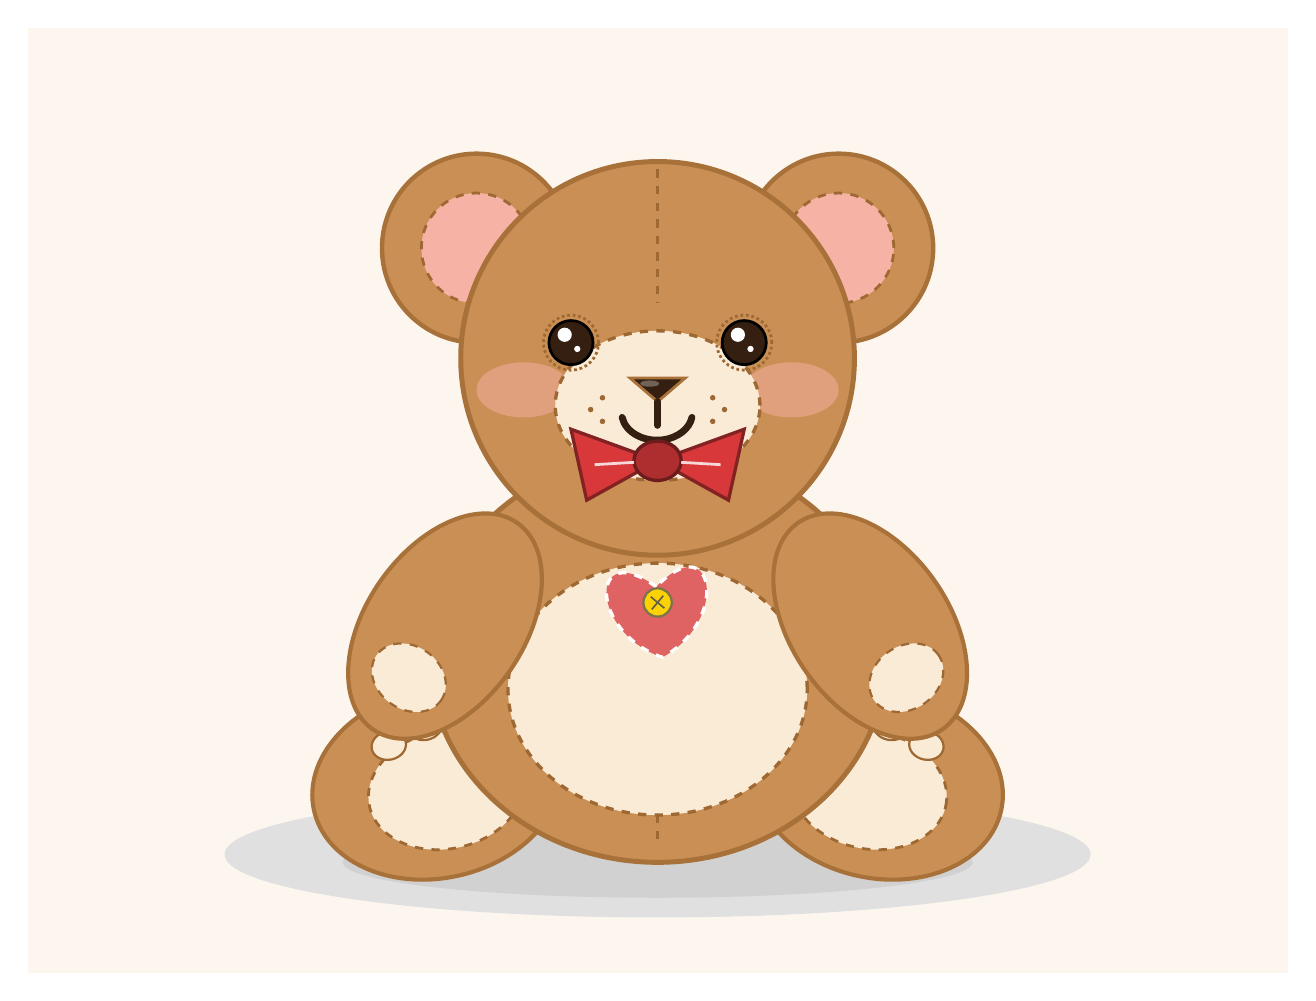
\begin{tikzpicture}[x=1cm, y=1cm]

  % Background canvas
  \fill[bgcream] (-8, -6) rectangle (8, 6);

  % Floor shadow
  \fill[black!12] (0, -4.5) ellipse (5.5 and 0.8);
  \fill[black!18] (0, -4.6) ellipse (4.0 and 0.45);

  % Back Legs / Feet (Sitting pose)
  % Left foot
  \begin{scope}[shift={(-2.8, -3.6)}, rotate=12]
    \filldraw[fill=bearbrown, draw=beardark, line width=1.5pt] (0,0) ellipse (1.6 and 1.2);
    \filldraw[fill=bearcream, draw=stitchcolor, dashed, line width=1pt] (0.1,-0.1) ellipse (1.0 and 0.75);
    \filldraw[fill=bearcream, draw=stitchcolor, line width=0.8pt] (-0.5, 0.6) ellipse (0.22 and 0.18);
    \filldraw[fill=bearcream, draw=stitchcolor, line width=0.8pt] (0.0, 0.75) ellipse (0.22 and 0.18);
    \filldraw[fill=bearcream, draw=stitchcolor, line width=0.8pt] (0.5, 0.65) ellipse (0.22 and 0.18);
  \end{scope}

  % Right foot
  \begin{scope}[shift={(2.8, -3.6)}, rotate=-12]
    \filldraw[fill=bearbrown, draw=beardark, line width=1.5pt] (0,0) ellipse (1.6 and 1.2);
    \filldraw[fill=bearcream, draw=stitchcolor, dashed, line width=1pt] (-0.1,-0.1) ellipse (1.0 and 0.75);
    \filldraw[fill=bearcream, draw=stitchcolor, line width=0.8pt] (0.5, 0.6) ellipse (0.22 and 0.18);
    \filldraw[fill=bearcream, draw=stitchcolor, line width=0.8pt] (0.0, 0.75) ellipse (0.22 and 0.18);
    \filldraw[fill=bearcream, draw=stitchcolor, line width=0.8pt] (-0.5, 0.65) ellipse (0.22 and 0.18);
  \end{scope}

  % Plump Torso
  \filldraw[fill=bearbrown, draw=beardark, line width=1.8pt] (0, -2.0) ellipse (2.9 and 2.6);

  % Center vertical body seam
  \draw[stitchcolor, dashed, line width=1.2pt] (0, -0.2) -- (0, -4.3);

  % Soft belly patch
  \filldraw[fill=bearcream, draw=stitchcolor, dashed, line width=1.2pt] (0, -2.4) ellipse (1.9 and 1.6);

  % Heart chest patch
  \begin{scope}[shift={(0, -1.3)}, rotate=5]
    \filldraw[fill=patchred, draw=white, dashed, line width=1.2pt]
      (0, 0.2) .. controls (-0.8, 0.9) and (-0.9, -0.3) .. (0, -0.7)
      .. controls (0.9, -0.3) and (0.8, 0.9) .. (0, 0.2) -- cycle;
    % Patch center button
    \filldraw[fill=yellow!70!orange, draw=yellow!40!black, line width=0.8pt] (0, 0) circle (0.18);
    \draw[yellow!30!black, line width=0.6pt] (-0.08, -0.08) -- (0.08, 0.08);
    \draw[yellow!30!black, line width=0.6pt] (-0.08, 0.08) -- (0.08, -0.08);
  \end{scope}

  % Short rounded arms
  % Left arm
  \begin{scope}[shift={(-2.7, -1.6)}, rotate=-35]
    \filldraw[fill=bearbrown, draw=beardark, line width=1.5pt] (0,0) ellipse (1.0 and 1.6);
    \filldraw[fill=bearcream, draw=stitchcolor, dashed, line width=0.8pt] (0, -0.8) ellipse (0.5 and 0.4);
  \end{scope}

  % Right arm
  \begin{scope}[shift={(2.7, -1.6)}, rotate=35]
    \filldraw[fill=bearbrown, draw=beardark, line width=1.5pt] (0,0) ellipse (1.0 and 1.6);
    \filldraw[fill=bearcream, draw=stitchcolor, dashed, line width=0.8pt] (0, -0.8) ellipse (0.5 and 0.4);
  \end{scope}

  % Ears (Symmetrical, round & large)
  % Left ear
  \filldraw[fill=bearbrown, draw=beardark, line width=1.6pt] (-2.3, 3.2) circle (1.2);
  \filldraw[fill=earpink, draw=stitchcolor, dashed, line width=1pt] (-2.3, 3.2) circle (0.7);

  % Right ear
  \filldraw[fill=bearbrown, draw=beardark, line width=1.6pt] (2.3, 3.2) circle (1.2);
  \filldraw[fill=earpink, draw=stitchcolor, dashed, line width=1pt] (2.3, 3.2) circle (0.7);

  % Big Round Head
  \filldraw[fill=bearbrown, draw=beardark, line width=1.8pt] (0, 1.8) circle (2.5);

  % Head vertical seam
  \draw[stitchcolor, dashed, line width=1.2pt] (0, 4.2) -- (0, 2.5);

  % Rosy cheeks
  \fill[earpink, opacity=0.5] (-1.7, 1.4) ellipse (0.6 and 0.35);
  \fill[earpink, opacity=0.5] (1.7, 1.4) ellipse (0.6 and 0.35);

  % Cream Muzzle
  \filldraw[fill=bearcream, draw=stitchcolor, dashed, line width=1.2pt] (0, 1.2) ellipse (1.3 and 0.95);

  % Glossy Button Eyes
  \foreach \x in {-1.1, 1.1} {
    \draw[stitchcolor, densely dotted, line width=1pt] (\x, 2.0) circle (0.35);
    \filldraw[fill=eyeblack, draw=black, line width=1pt] (\x, 2.0) circle (0.28);
    \fill[white] (\x-0.08, 2.1) circle (0.09);
    \fill[white] (\x+0.08, 1.92) circle (0.04);
  }

  % Soft Stitched Nose
  \filldraw[fill=eyeblack, draw=beardark, line width=1pt]
    (-0.35, 1.55) -- (0.35, 1.55) -- (0, 1.25) -- cycle;
  \fill[white!30!eyeblack] (-0.1, 1.48) ellipse (0.12 and 0.04);

  % Embroidered Mouth
  \draw[eyeblack, line width=2.5pt, line cap=round] (0, 1.25) -- (0, 0.95);
  \draw[eyeblack, line width=2.5pt, line cap=round]
    (-0.45, 1.05) arc (190:350:0.45 and 0.35);

  % Whiskers/freckles dots
  \foreach \pos in {(-0.7, 1.3), (-0.85, 1.15), (-0.7, 1.0), (0.7, 1.3), (0.85, 1.15), (0.7, 1.0)} {
    \fill[stitchcolor] \pos circle (0.035);
  }

  % Red Neck Bow
  \filldraw[fill=ribbonred, draw=ribbonred!60!black, line width=1.2pt]
    (0, 0.5) -- (-1.1, 0.9) -- (-0.9, 0.0) -- cycle;
  \filldraw[fill=ribbonred, draw=ribbonred!60!black, line width=1.2pt]
    (0, 0.5) -- (1.1, 0.9) -- (0.9, 0.0) -- cycle;
  \filldraw[fill=ribbonred!80!black, draw=ribbonred!50!black, line width=1.2pt]
    (0, 0.5) ellipse (0.3 and 0.25);
  \draw[white!80!ribbonred, line width=1pt] (-0.8, 0.45) -- (-0.3, 0.48);
  \draw[white!80!ribbonred, line width=1pt] (0.8, 0.45) -- (0.3, 0.48);

\end{tikzpicture}
\end{document}
